%============== PREAMBOLO E DICHIARAZIONI INIZIALI ==========
\documentclass[10pt,oneside,a4paper]{article}

\usepackage[latin1]{inputenc} 
\usepackage[italian]{babel}
\usepackage{siunitx} %Inserisce automaticamente i dati con le unit� di misura correttamente formattate del SI (utilizzo: \SI{0.82}{m^2}, in generale \SI{misura con il punto decimale}{unit� di misura})
\sisetup{output-decimal-marker = {.}, separate-uncertainty = true, input-uncertainty-signs = \pm, detect-weight=true, detect-family=true} %per usare SI con la virgola decimale
\usepackage{listings} %Per citare codice informatico formattandolo correttamente
\usepackage{amsmath}
\usepackage{graphicx}
\usepackage{epigraph}
\usepackage{booktabs}	%tabelle migliorate
\usepackage{tablefootnote}	%note a pi� di pagina in tabella
\usepackage{threeparttable} %tabella con note a pi� di tabella
\usepackage{caption}	%descrizione per figure
\captionsetup{tableposition=top,figureposition=bottom,font=small} %setup descrizione
\usepackage{float}
\usepackage{esvect} %vettori
\usepackage{longtable} %tabelle lunghe

\setcounter{section}{-1}

%========= PRIMA PAGINA ===========
\title{\textsc{Misura della costante elastica di una molla e dell'accelerazione di gravit� }}
\author{\small{G. Galbato Muscio} \and \small{L. Gravina} \and \small{L. Graziotto} \and \small{M. Rescigno}}
\date{}

\begin{document}
\begin{figure}
	\centering
	\includegraphics[scale=0.5,trim={2.8cm 8.9cm 0 9cm},clip]{logo.png}
\end{figure}
\maketitle
\begin{center} 
\fbox{{\fontsize{13pt}{8mm}\textsc{Gruppo B2.3}}} \\
\vspace{1cm}
\begin{tabular}{ccc}
	 Esperienza di laboratorio && Consegna della relazione \\
	  \emph{\small{6 aprile 2017}} && \emph{\small{11 aprile 2017}} \\
\end{tabular} 

\vspace{0.5cm}

\end{center}
\hrule
\vspace{0.5cm}
\begin{abstract}
L'accelerazione di gravit� $g$ influenza il moto oscillatorio di una massa appesa ad una molla. Studiando il periodo e l'allungamento di essa, ne calcoliamo la costante elastica $k$ e stimiamo $g$.
\end{abstract}
\vspace{0.5cm}
\newpage
\tableofcontents %Indice
\listoftables %Indice delle tabelle
\listoffigures %Indice dei grafici
\pagebreak
\section{Convenzioni e formule}
In questa relazione verranno usate le seguenti convenzioni:
\begin{enumerate}
	\item sar� usato il punto [ $.$ ] come separatore decimale;
	\item l'approssimazione decimale della cifra $5$ sar� fatta per eccesso;
	\item al fine di migliorare la qualit� dell'elaborazione dei dati, ogni grafico/istogramma prodotto a mano su carta millimetrata sar� riportato insieme al suo equivalente prodotto attraverso un software di analisi dati\footnote{In questo contesto i dati sono stati elaborati con il software di analisi \emph{R}.};
	\item al fine di snellire la relazione e migliorarne la leggibilit�, riporteremo nel corpo del documento solamente le tabelle riepilogative e dedicheremo un'appendice finale alle tabelle contenenti tutte le singole misure e i singoli risultati. 
\end{enumerate}
Inoltre, si far� riferimento alle seguenti formule:
\begin{enumerate}
	\item media 
		\begin{equation}\label{eq:media}
			\bar{x} = \frac{1}{N}\sum_{i=1}^Nx_i;
		\end{equation}
	\item varianza
		\begin{equation}\label{eq:varianza}
			\sigma^2 = \frac{1}{N}\sum_{i=1}^N(x_i-\bar{x})^2;
		\end{equation}
	\item deviazione standard
		\begin{equation}\label{eq:deviazione}
			\sigma = \sqrt{\sigma^2}.
		\end{equation}	
\end{enumerate}

%===============SCOPO E DESCRIZIONE DELL'ESPERIENZA==============
\section{Scopo e descrizione dell'esperienza}
\label{sec:description}
Una molla di costante elastica $k$ a cui � attaccata una massa $m$ soggetta alla forza peso $m\vec{g}$, reagisce con una forza data dalla \textbf{Legge di Hooke} $F=-k(x-x_0)$, e si porta nella posizione di equilibrio $x_{\text{eq}}=x_0+mg/k$; spostando la massa dalla posizione di equilibrio, si origina un moto armonico di periodo $T=2\pi\sqrt{m/k}$.

In questa esperienza calcoliamo in modo indiretto la costante elastica $k$ della molla a partire dalle misure del periodo di oscillazione, e misurando la posizione di equilibrio in funzione della massa applicata, stimiamo la costante di accelerazione gravitazionale $g$. 

Adottiamo due metodi diversi:
\begin{enumerate}
\item misuriamo ripetutamente periodo e allungamento e dai valori medi calcoliamo $k$ e $g$;
\item misuriamo il periodo e l'allungamento in funzione della massa applicata e, graficamente, ricaviamo i coefficienti di proporzionalit� tra determinati valori che ci consentono di estrarre $k$ e $g$.
\end{enumerate}

%================APPARATO SPERIMENTALE======================
\section{Apparato Sperimentale}

\subsection{Strumenti}
\label{subsec:strumenti}
\begin{itemize}
\item Molla appesa ad un supporto con carta millimetrata per misurarne l'allungamento [divisione \SI{1}{mm}, incertezza \SI{0,3}{mm}];
\item Bilancia per la misura della massa dei campioni [risoluzione \SI{0,1}{g}, incertezza \SI{0,03}{g}, portata \SI{2000}{g}];
\item Cronometro a lettura digitale per le misure di periodo [risoluzione \SI{0,01}{s}, incertezza \SI{0,003}{s}];
\item Squadra per ridurre l'errore di parallasse nella misura di allungamento.
\end{itemize}

\subsection{Campioni}
\label{subsec:campioni}
\begin{itemize}
\item $10$ dischetti che si possono appendere alla molla.
\end{itemize}

%==============SEQUENZA OPERAZIONI SPERIMENTALI============
\section{Sequenza Operazioni Sperimentali}

\subsection{Verifica degli strumenti}
\label{subsec:verifica}
Per quanto riguarda la molla, notiamo che applicando meno di tre dischetti questa non si deforma, dunque non possiamo compiere misure di allungamento o di periodo in tale circostanza (il problema sar� meglio trattato nel paragrafo~\ref{subsec:metodo2}). Inoltre scegliamo di adottare un'incertezza di \SI{0,3}{mm} per l'allungamento in quanto non riusciamo a interpolare tra meno di mezza tacca: la nostra risoluzione � dunque \SI{0,5}{mm} e l'incertezza � pari a $\SI{0,5}{mm}/\sqrt{3}=\SI{0,3}{mm}$. La bilancia pu� essere tarata prima di ogni misurazione e assumiamo come incertezza $0,3$ volte la sua risoluzione. La misura del periodo non � compromessa dal tempo di reazione dello sperimentatore nell'azionare il cronometro in quanto stimiamo che l'intervallo tra l'inizio del fenomeno e la partenza del cronometro sia pari a quello tra la fine del fenomeno e lo stop del cronometro.

%============== METODO 1 ================================
\subsection{Metodo 1}
\label{subsec:metodo1}
Misuriamo la massa complessiva di $5$ dischetti e quindi di tutti i $10$ dischetti con la bilancia, e quindi l'allungamento della molla a cui essi sono applicati, ripetendo in entrambi i casi le misure $5$ volte. Eseguiamo poi $50$ misure ripetute di $5$ periodi di oscillazione e successivamente $5$ misure ripetute di $50$ periodi di oscillazione, applicando sia $5$ dischetti sia $10$ dischetti.

I dati sperimentali sono riportati nelle tabelle~\ref{tab:metodo1_allungamento-massa},\ref{tab:5periodi_5dischi},\ref{tab:5periodi_10dischi},\ref{tab:50periodi_5dischi} e \ref{tab:50periodi_10dischi}, e negli istogrammi di figure~\ref{fig:ist_5dischi} e \ref{fig:ist_10dischi}.


%============= METODO 2 =================================
\subsection{Metodo 2}
\label{subsec:metodo2}
Adottiamo ora un metodo grafico per ricavare $k$ e $g$: misuriamo in modo integrale la massa dei dischetti e dunque l'allungamento della molla aggiungendoli progressivamente. Eseguiamo al contempo per ogni campione aggiunto $20$ misure ripetute del tempo impiegato per compiere $10$ oscillazioni (i dati sperimentali raccolti sono riportati nelle tabelle~\ref{tab:metodo2_allungamento-massa} e \ref{tab:metodo2_periodo}). 

Poich� il quadrato del periodo di oscillazione e l'allungamento della molla sono direttamente proporzionali alla massa appesa ad essa, secondo coefficienti di proporzionalit� legati alle costanti oggetto di indagine, in particolare
	\begin{align*}
	T^2 &= T_0^2 + \alpha_1 m \\
	x &= \bar{x_0} + \alpha_2 m,
	\end{align*}
tracciamo il grafico (figura~\ref{fig:periodoquadro-massa}) di $T^2$ in funzione della massa $m$, e quello (figura~\ref{fig:xeq-massa}) dell'allungamento in funzione della massa $m$. Estraiamo dunque i coefficienti angolari delle rette che meglio approssimano i punti sperimentali, chiamati rispettivamente $\alpha_1$ e $\alpha_2$. Noti tali valori, possiamo calcolare la costante elastica dall'equazione
	\[
	k = \frac{4\pi^2}{\alpha_1}
	\]
e l'accelerazione gravitazionale da
	\[
	g = 4\pi^2\frac{\alpha_2}{\alpha_1}.
	\]

Per il calcolo di $\alpha_1$, scegliamo sulla retta interpolatrice (figura~\ref{fig:periodoquadro-massa}) i seguenti punti
	\begin{align*}
	m_1 = \SI{180.00}{g}, \qquad & T^2_1 = \SI{0.20}{s^2}; \\
	m_2 = \SI{810.00}{g}, \qquad & T^2_2 = \SI{0.76}{s^2};
	\end{align*}
dunque $\alpha_1 = \SI{8.88\pm0.02 e-4}{s^2/g}$. L'incertezza su questo valore � stata valutata ricordando che stiamo calcolando il rapporto tra $\Delta(T^2) = (T^2)_2 - (T^2)_1$ e $\Delta m = m_2 - m_1$, dunque si ha
	\[
	\sigma_{\alpha_1} = \sqrt{\left(\frac{\sigma_{\Delta (T^2)}}{\Delta(T^2)}\right)^2 + \left(\frac{\sigma_{\Delta m}}{\Delta m}\right)^2} \cdot \alpha_1,
	\]
dove 
	\[
	\sigma^2_{\Delta(T^2)} = (2T_2\delta_{T_2})^2 + (2T_1\delta_{T_1})^2,
	\]
usando come incertezza sul periodo $\delta_T = \sqrt{(\sigma_T/\sqrt{20})^2 + u_T^2} / 10$ (con $\sigma_T$ la deviazione standard del punto sperimentale pi� vicino al punto della retta scelto e $u_T$ l'incertezza strumentale sul periodo), e 
	\[
	\sigma^2_{\Delta m} = 2\sigma_m^2
	\] 
(con $\sigma_m$ l'incertezza strumentale sulla massa).		
Perci� otteniamo la costante elastica della molla
	\[
	\boxed{\textbf{$k$ = {\SI{44.4 \pm 0.1}{\frac{N}{m}}}}},
	\]
dove l'incertezza � stata valutata con l'equazione 
	\[
	\sigma_k = \frac{4\pi^2}{\alpha_1^2}\cdot \sigma_{\alpha_1}.
	\]
	
Per il calcolo di $\alpha_2$, scegliamo invece sulla retta interpolatrice (figura~\ref{fig:xeq-massa}) i seguenti punti
	\begin{align*}
	m_1 = \SI{270.00}{g}, \qquad & x_1 = \SI{15.0}{mm}; \\
	m_2 = \SI{800.00}{g}, \qquad & x_2 = \SI{129.0}{mm};
	\end{align*}
dunque $\alpha_2 = \SI{215.1 \pm 0.9}{\frac{mm}{g}}$. Analogamente al caso precedente, l'incertezza su questo valore � stata calcolata con
	\[
	\sigma_{\alpha_2} = \sqrt{\left(\frac{\sigma_{\Delta x}}{\Delta x}\right)^2 + \left(\frac{\sigma_{\Delta m}}{\Delta m}\right)^2} \cdot \alpha_2,
	\]
dove $\Delta x = x_2 - x_1$, $\Delta m = m_2 - m_1$, l'incertezza su $\Delta m$ � la medesima usata nel calcolo sopra e 
	\[
	\sigma_{\Delta x} = \sqrt{2 \delta^2_x},
	\]
con $\delta_x = \sqrt{\left(\frac{\sigma_x}{\sqrt{5}}\right)^2 + u_x^2}$, indicando con $\sigma_x$ la deviazione standard sulle $5$ misure di allungamento eseguite per ogni campione e con $u_x$ l'incertezza di lettura sulla carta millimetrata.
Otteniamo quindi l'accelerazione di gravit�
	\[
	\boxed{\textbf{$g$ = {\SI{9.55 \pm 0.04}{\frac{m}{s^2}}}}},
	\]
dove l'incertezza � stata propagata con l'equazione
	\[
	\sigma_g = \sqrt{\left(\frac{\alpha_2}{\alpha_1^2}\sigma_{\alpha_1}\right)^2 + \left(\frac{4\pi^2}{\alpha_1}\sigma_{\alpha_2}\right)^2}.
	\]

Riteniamo che la causa principale della discrepanza dei valori trovati con i \emph{valori veri} provenga dalla qualit� della nostra interpolazione manuale; infatti, utilizzando l'algoritmo di interpolazione del software \emph{R}, ricaviamo valori pi� precisi dei coefficienti angolari, da cui si ottengono (assumendo le medesime incertezze calcolate poc'anzi) 
	\begin{align*}
	k &= \SI{45.8 \pm 0.1}{\frac{N}{m}} \\
	g &= \SI{9.84 \pm 0.04}{\frac{m}{s^2}},
	\end{align*} 
ove osserviamo che l'accelerazione di gravit� � in accordo con il valore vero di~\SI{9.81}{\frac{m}{s^2}}.

Infine, sottolineiamo che con meno di tre dischetti appesi alla molla non � stato possibile compiere misure n� di allungamento n� di periodo, in quanto essa non si � deformata: deduciamo che appendendo uno o due dischetti ci troviamo al di sotto della \emph{soglia di discriminazione}, per cui la molla non reagisce allo stimolo applicato.


%============= CONSIDERAZIONI FINALI ====================
\section{Considerazioni finali}
\label{sec:c_finali}

%============= TABELLE e GRAFICI =======================
\newpage
\section{Appendice: tabelle e grafici}
\subsection{Tabelle metodo 1}

\begin{table}[ht]
\caption{Allungamento della molla rispetto alla posizione di equilibro iniziale in seguito al posizionamento dei dischetti}
\label{tab:allungamento}
\centering
\begin{tabular}{ccc}
  \hline
 & Allungamento 5 dischetti [mm] & Allungamento 10 dischetti [mm] \\ 
&($\pm$0.5) & ($\pm$0.5)\\
  \hline
1 & 42.0 & 125.0 \\ 
  2 & 41.0 & 123.5 \\ 
  3 & 41.5 & 124.5 \\ 
  4 & 41.0 & 123.5 \\ 
  5 & 41.0 & 125.5 \\ 
   \hline
\end{tabular}
\end{table}


\begin{center}
\begin{longtable}{ccccc}
\label{tab:periodi}\\
\caption{50 misure del periodo di 5 oscillazioni della molla sottoposta a pesi differenti}\\
\hline
 osservazioni & 5 dischi & 5 dischi & 10 dischi & 10 dischi \\
  & 5 oscillazioni & 1 oscillazione & 5 oscillazioni & 1 oscillazione \\
  & ($\pm$0.003) & ($\pm$0.003) &($\pm$0.003) & ($\pm$0.003)\\
\hline
\endfirsthead
\multicolumn{5}{c}%
{\tablename\ \thetable\ -- \textit{Continued from previous page}} \\
\hline
First entry & Second entry & Third entry & Fourth entry & Fourth entry \\
\hline
\endhead
\hline \multicolumn{5}{r}{\textit{Continued on next page}} \\
\endfoot
\hline
\endlastfoot
1 & 3.100 & 0.620 & 4.270 & 0.854 \\ 
  2 & 3.170 & 0.634 & 4.310 & 0.862 \\ 
  3 & 3.370 & 0.674 & 4.240 & 0.848 \\ 
  4 & 3.190 & 0.638 & 4.230 & 0.846 \\ 
  5 & 3.050 & 0.610 & 4.190 & 0.838 \\ 
  6 & 3.100 & 0.620 & 4.230 & 0.846 \\ 
  7 & 3.110 & 0.622 & 4.230 & 0.846 \\ 
  8 & 3.270 & 0.654 & 4.230 & 0.846 \\ 
  9 & 3.100 & 0.620 & 4.210 & 0.842 \\ 
  10 & 3.130 & 0.626 & 4.220 & 0.844 \\ 
  11 & 3.130 & 0.626 & 4.140 & 0.828 \\ 
  12 & 3.130 & 0.626 & 4.230 & 0.846 \\ 
  13 & 3.130 & 0.626 & 4.170 & 0.834 \\ 
  14 & 3.150 & 0.630 & 4.260 & 0.852 \\ 
  15 & 3.150 & 0.630 & 4.190 & 0.838 \\
  6 & 3.170 & 0.634 & 4.220 & 0.844 \\ 
  17 & 3.250 & 0.650 & 4.220 & 0.844 \\ 
  18 & 3.110 & 0.622 & 4.170 & 0.834 \\ 
  19 & 3.070 & 0.614 & 4.220 & 0.844 \\ 
  20 & 3.100 & 0.620 & 4.230 & 0.846 \\ 
  21 & 3.070 & 0.614 & 4.190 & 0.838 \\ 
  22 & 3.190 & 0.638 & 4.230 & 0.846 \\ 
  23 & 3.100 & 0.620 & 4.190 & 0.838 \\ 
  24 & 3.120 & 0.624 & 4.250 & 0.850 \\ 
  25 & 3.090 & 0.618 & 4.230 & 0.846 \\ 
  26 & 3.100 & 0.620 & 4.230 & 0.846 \\ 
  27 & 3.070 & 0.614 & 4.230 & 0.846 \\ 
  28 & 3.070 & 0.614 & 4.260 & 0.852 \\ 
  29 & 3.100 & 0.620 & 4.290 & 0.858 \\
  30 & 3.130 & 0.626 & 4.250 & 0.850 \\
  31 & 3.020 & 0.604 & 4.190 & 0.838 \\ 
  32 & 3.070 & 0.614 & 4.250 & 0.850 \\ 
  33 & 3.080 & 0.616 & 4.230 & 0.846 \\ 
  34 & 3.070 & 0.614 & 4.190 & 0.838 \\ 
  35 & 3.080 & 0.616 & 4.240 & 0.848 \\ 
  36 & 3.070 & 0.614 & 4.220 & 0.844 \\ 
  37 & 3.090 & 0.618 & 4.230 & 0.846 \\ 
  38 & 3.120 & 0.624 & 4.230 & 0.846 \\ 
  39 & 3.110 & 0.622 & 4.270 & 0.854 \\ 
  40 & 3.160 & 0.632 & 4.190 & 0.838 \\ 
  41 & 3.030 & 0.606 & 4.250 & 0.850 \\ 
  42 & 3.100 & 0.620 & 4.180 & 0.836 \\ 
  43 & 3.100 & 0.620 & 4.170 & 0.834 \\ 
  44 & 3.020 & 0.604 & 4.200 & 0.840 \\ 
  45 & 3.030 & 0.606 & 4.200 & 0.840 \\ 
  46 & 3.090 & 0.618 & 4.250 & 0.850 \\ 
  47 & 3.030 & 0.606 & 4.230 & 0.846 \\ 
  48 & 3.030 & 0.606 & 4.270 & 0.854 \\ 
  49 & 3.090 & 0.618 & 4.190 & 0.838 \\ 
  50 & 3.090 & 0.618 & 4.250 & 0.850 \\ 
\end{longtable}
\end{center}

\begin{table}[ht]
\caption{5 misure del periodo di 50 oscillazioni della molla sottoposta a pesi differenti}
\label{tab:allungamento}
\centering
\begin{tabular}{ccccc}
  \hline
 & 5 dischi & 5 dischi & 10 dischi & 10 dischi\\
 & 50 oscillazioni  & 1 oscillazione  & 50 oscillazioni  & 1 oscillazione\\
 & ($\pm$0.003) & ($\pm$0.003) &($\pm$0.003) & ($\pm$0.003)\\
  \hline
1 & 30.670 & 0.613 & 42.110 & 0.842 \\ 
  2 & 30.690 & 0.614 & 42.160 & 0.843 \\ 
  3 & 30.600 & 0.612 & 41.920 & 0.838 \\ 
  4 & 30.610 & 0.612 & 41.930 & 0.839 \\ 
  5 & 30.690 & 0.614 & 42.140 & 0.843 \\ 
   \hline
\end{tabular}
\end{table}



\begin{table}[ht]
\caption{K e g ricavate da 5 misure di 50 oscillazioni}
\label{tab:k_g}
\centering
\begin{tabular}{ccc}
  \hline
 & K 50 oscillazioni & g 50 oscillazioni \\ 
  \hline
1 & 46.8 & 9.84 \\ 
  2 & 46.6 & 9.74 \\ 
  3 & 47.5 & 9.98 \\ 
  4 & 47.5 & 9.92 \\ 
  5 & 46.7 & 10.00 \\ 
   \hline
\end{tabular}
\end{table}




\begin{center}
\begin{longtable}{ccccc}
\label{tab:K_g2}\\
\caption{K e g ricavate da 50 misure di 5 oscillazioni}\\
\hline
 $\quad$ & $\quad$K$\quad$ & $\quad$g$\quad$\\
  & ($\pm$0.?) & ($\pm$0.0?) \\
\hline
\endfirsthead
\multicolumn{3}{c}%
{\tablename\ \thetable\ -- \textit{Continued from previous page}} \\
\hline
First entry & Second entry & Third entry\\
\hline
\endhead
\hline \multicolumn{3}{r}{\textit{Continued on next page}} \\
\endfoot
\hline
\endlastfoot
\hline
1 & 45.2 & 9.50 \\ 
  2 & 45.7 & 9.55 \\ 
  3 & 58.9 & 12.37 \\ 
  4 & 50.5 & 10.55 \\ 
  5 & 47.2 & 10.10 \\ 
  6 & 47.1 & 9.89 \\ 
  7 & 47.4 & 9.90 \\ 
  8 & 54.1 & 11.38 \\ 
  9 & 48.0 & 10.03 \\ 
  10 & 48.6 & 10.41 \\ 
  11 & 53.1 & 11.16 \\ 
  12 & 48.1 & 10.06 \\ 
  13 & 51.3 & 10.79 \\ 
  14 & 47.4 & 9.90 \\ 
  15 & 51.1 & 10.93 \\ 
  16 & 50.2 & 10.56 \\ 
  17 & 53.8 & 11.24 \\ 
  18 & 50.5 & 10.62 \\ 
  19 & 46.5 & 9.71 \\ 
  20 & 47.1 & 10.07 \\ 
  21 & 47.9 & 10.07 \\ 
  22 & 50.5 & 10.55 \\ 
  23 & 49.0 & 10.31 \\ 
  24 & 46.8 & 9.78 \\ 
  25 & 46.7 & 9.99 \\ 
  26 & 47.1 & 9.89 \\ 
  27 & 46.0 & 9.62 \\ 
  28 & 44.7 & 9.39 \\ 
  29 & 44.3 & 9.26 \\ 
  30 & 47.2 & 10.09 \\ 
  31 & 46.2 & 9.71 \\ 
  32 & 45.1 & 9.43 \\ 
  33 & 46.4 & 9.74 \\ 
  34 & 47.9 & 10.01 \\ 
  35 & 45.9 & 9.82 \\ 
  36 & 46.5 & 9.77 \\ 
  37 & 46.7 & 9.76 \\ 
  38 & 47.8 & 10.04 \\ 
  39 & 45.5 & 9.51 \\ 
  40 & 51.5 & 11.02 \\ 
  41 & 43.9 & 9.22 \\ 
  42 & 49.6 & 10.36 \\ 
  43 & 50.1 & 10.53 \\ 
  44 & 45.7 & 9.56 \\ 
  45 & 46.1 & 9.86 \\ 
  46 & 45.8 & 9.62 \\ 
  47 & 44.7 & 9.35 \\ 
  48 & 43.1 & 9.05 \\ 
  49 & 48.7 & 10.17 \\ 
  50 & 45.8 & 9.79 \\ 
  \hline
\end{longtable}
\end{center}

\begin{figure}
\begin{center}
\caption{Metodo grafico: $T^2$ in funzione di $m$ e retta di \emph{best fit}}
\label{fig:periodoquadro-massa}
\includegraphics[scale=0.18]{Tquadrovsmassa.png}
\end{center}
\end{figure}

\begin{figure}
\begin{center}
\caption{Metodo grafico: $T^2$ in funzione di $m$ e retta di \emph{best fit} generato con \emph{R}}
\label{fig:periodoquadro-massa-R}
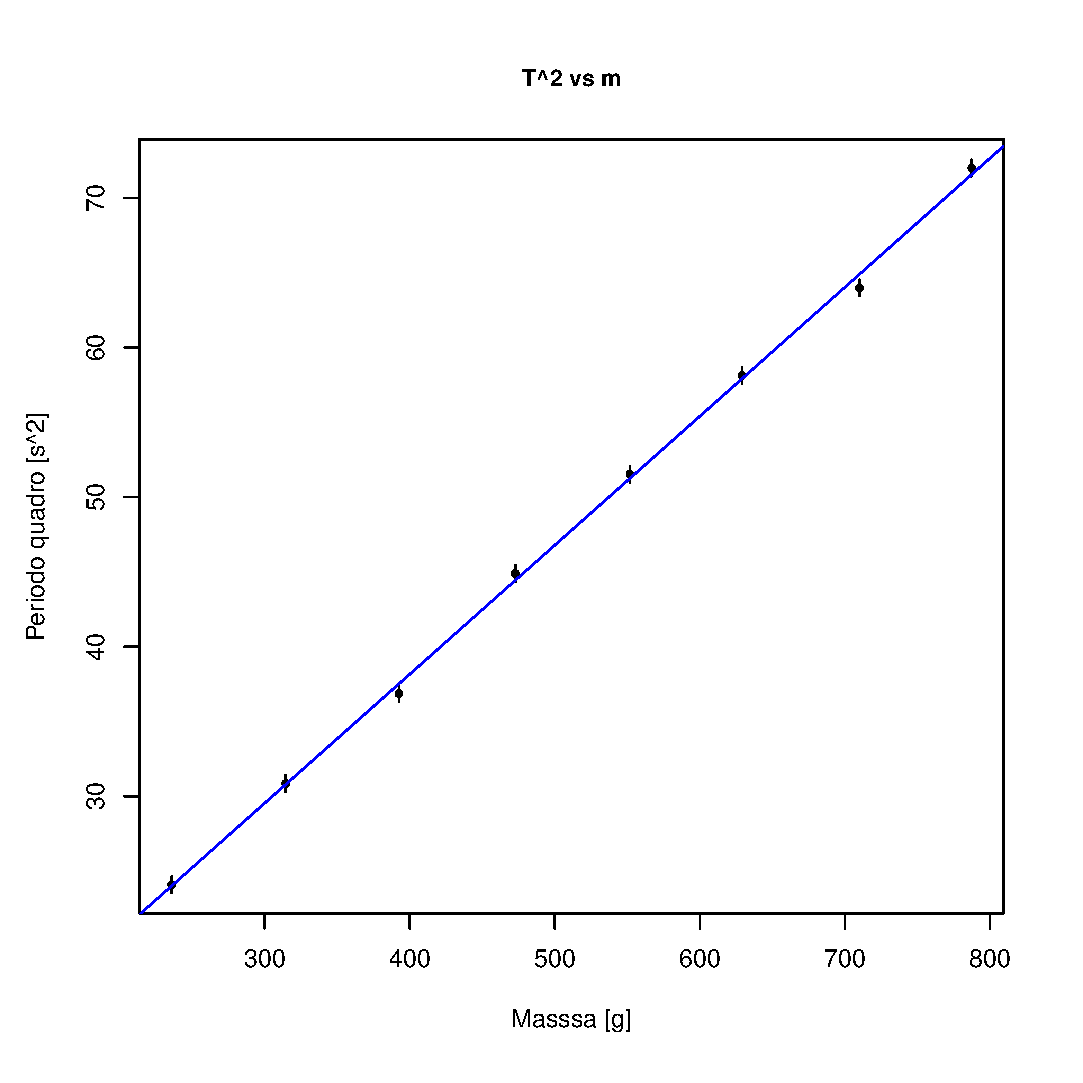
\includegraphics[scale=0.5]{metodo_grafico_1.eps}
\end{center}
\end{figure}

\begin{figure}
\begin{center}
\caption{Metodo grafico: $x_\text{eq}$ in funzione di $m$ e retta di \emph{best fit}}
\label{fig:xeq-massa}
\includegraphics[scale=0.18]{xeqvsmassa.png}
\end{center}
\end{figure}

\begin{figure}
\begin{center}
\caption{Metodo grafico: $x_\text{eq}$ in funzione di $m$ e retta di \emph{best fit} generato con \emph{R}}
\label{fig:xeq-massa-R}
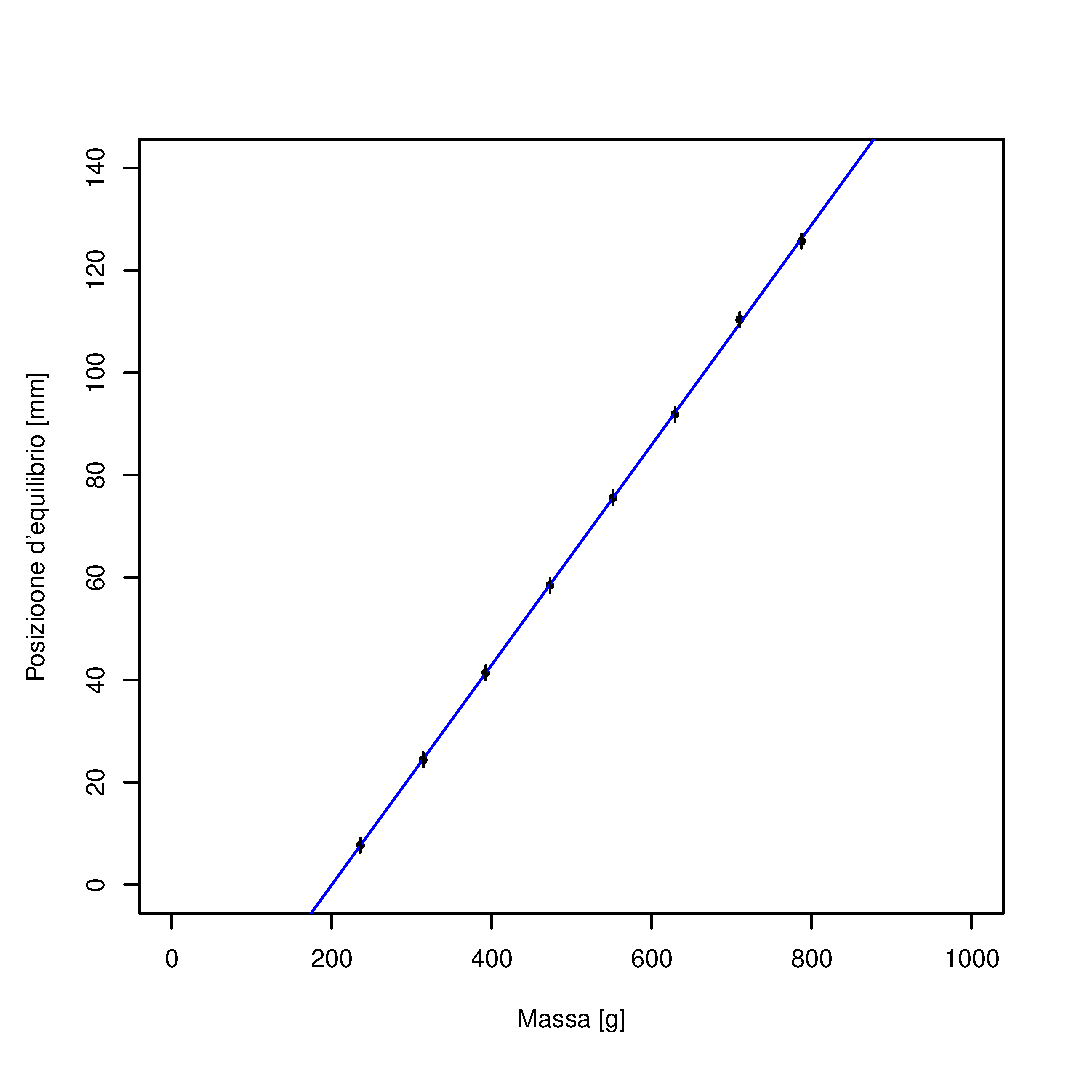
\includegraphics[scale=0.5]{metodo_grafico_2.eps}
\end{center}
\end{figure}




\end{document}
